% Kết quả tổng hợp từ 18 lượt train; độ lệch chuẩn là SD mẫu.
\section{Kết quả trên tập test}

Bảng~\ref{tab:new-image-results} tổng hợp accuracy và macro-F1 trên 9.998 ảnh trong tập test sau khi loại trùng pixel chính xác. Ở cả hai kiến trúc, chế độ partial vượt head-only; full tiếp tục cải thiện kết quả. ResNet18 full đạt $79{,}16\pm0{,}39$\%, còn Swin-T full đạt $86{,}81\pm0{,}02$\%.

\begin{table}[htbp]\centering\small
\setlength{\tabcolsep}{5pt}
\begin{tabular}{lrr}
\toprule
Cấu hình & Accuracy test (\%) & Macro-F1\\\midrule
ResNet18 head-only & $60{,}91\pm0{,}14$ & $0{,}6077\pm0{,}0012$\\
ResNet18 partial & $73{,}84\pm0{,}23$ & $0{,}7382\pm0{,}0018$\\
ResNet18 full & $79{,}16\pm0{,}39$ & $0{,}7915\pm0{,}0038$\\
Swin-T head-only & $71{,}69\pm0{,}07$ & $0{,}7156\pm0{,}0008$\\
Swin-T partial & $78{,}44\pm0{,}16$ & $0{,}7837\pm0{,}0015$\\
Swin-T full & $86{,}81\pm0{,}02$ & $0{,}8681\pm0{,}0001$\\
\bottomrule
\end{tabular}
\caption{Full cho accuracy cao nhất trong từng kiến trúc. Swin-T full đạt 86,81\% so với 79,16\% của ResNet18 full, cao hơn 7,66 điểm phần trăm theo so sánh ghép cặp cùng seed. Accuracy và macro-F1 được trình bày dưới dạng trung bình $\pm$ SD mẫu qua seed 42, 43 và 44.}
\label{tab:new-image-results}
\end{table}

Mức tăng khi mở thêm backbone khác nhau giữa hai kiến trúc. Với ResNet18, phần cải thiện lớn hơn xuất hiện từ head-only sang partial; với Swin-T, bước từ partial sang full đem lại mức tăng lớn hơn bước từ head-only sang partial. Như vậy, cập nhật riêng khối cuối chưa khai thác hết chất lượng đạt được của Swin-T trong ngân sách này. Tuy nhiên, các kết quả không xác định được tầng nào tạo ra mức cải thiện, cũng không cho phép quy toàn bộ lợi thế của Swin-T cho self-attention, vì kiến trúc và trọng số pretrained cùng thay đổi.

Accuracy và macro-F1 cho cùng thứ tự xếp hạng ở cả sáu cấu hình. Điều này cho thấy kết luận về cấu hình tốt hơn không phụ thuộc vào việc dùng tỷ lệ dự đoán đúng hay F1 trung bình theo lớp. Hai chỉ số gần nhau không có nghĩa mọi lớp đều dễ phân loại như nhau; sự khác biệt giữa các lớp cần được xem qua confusion matrix.

\begin{figure}[htbp]\centering
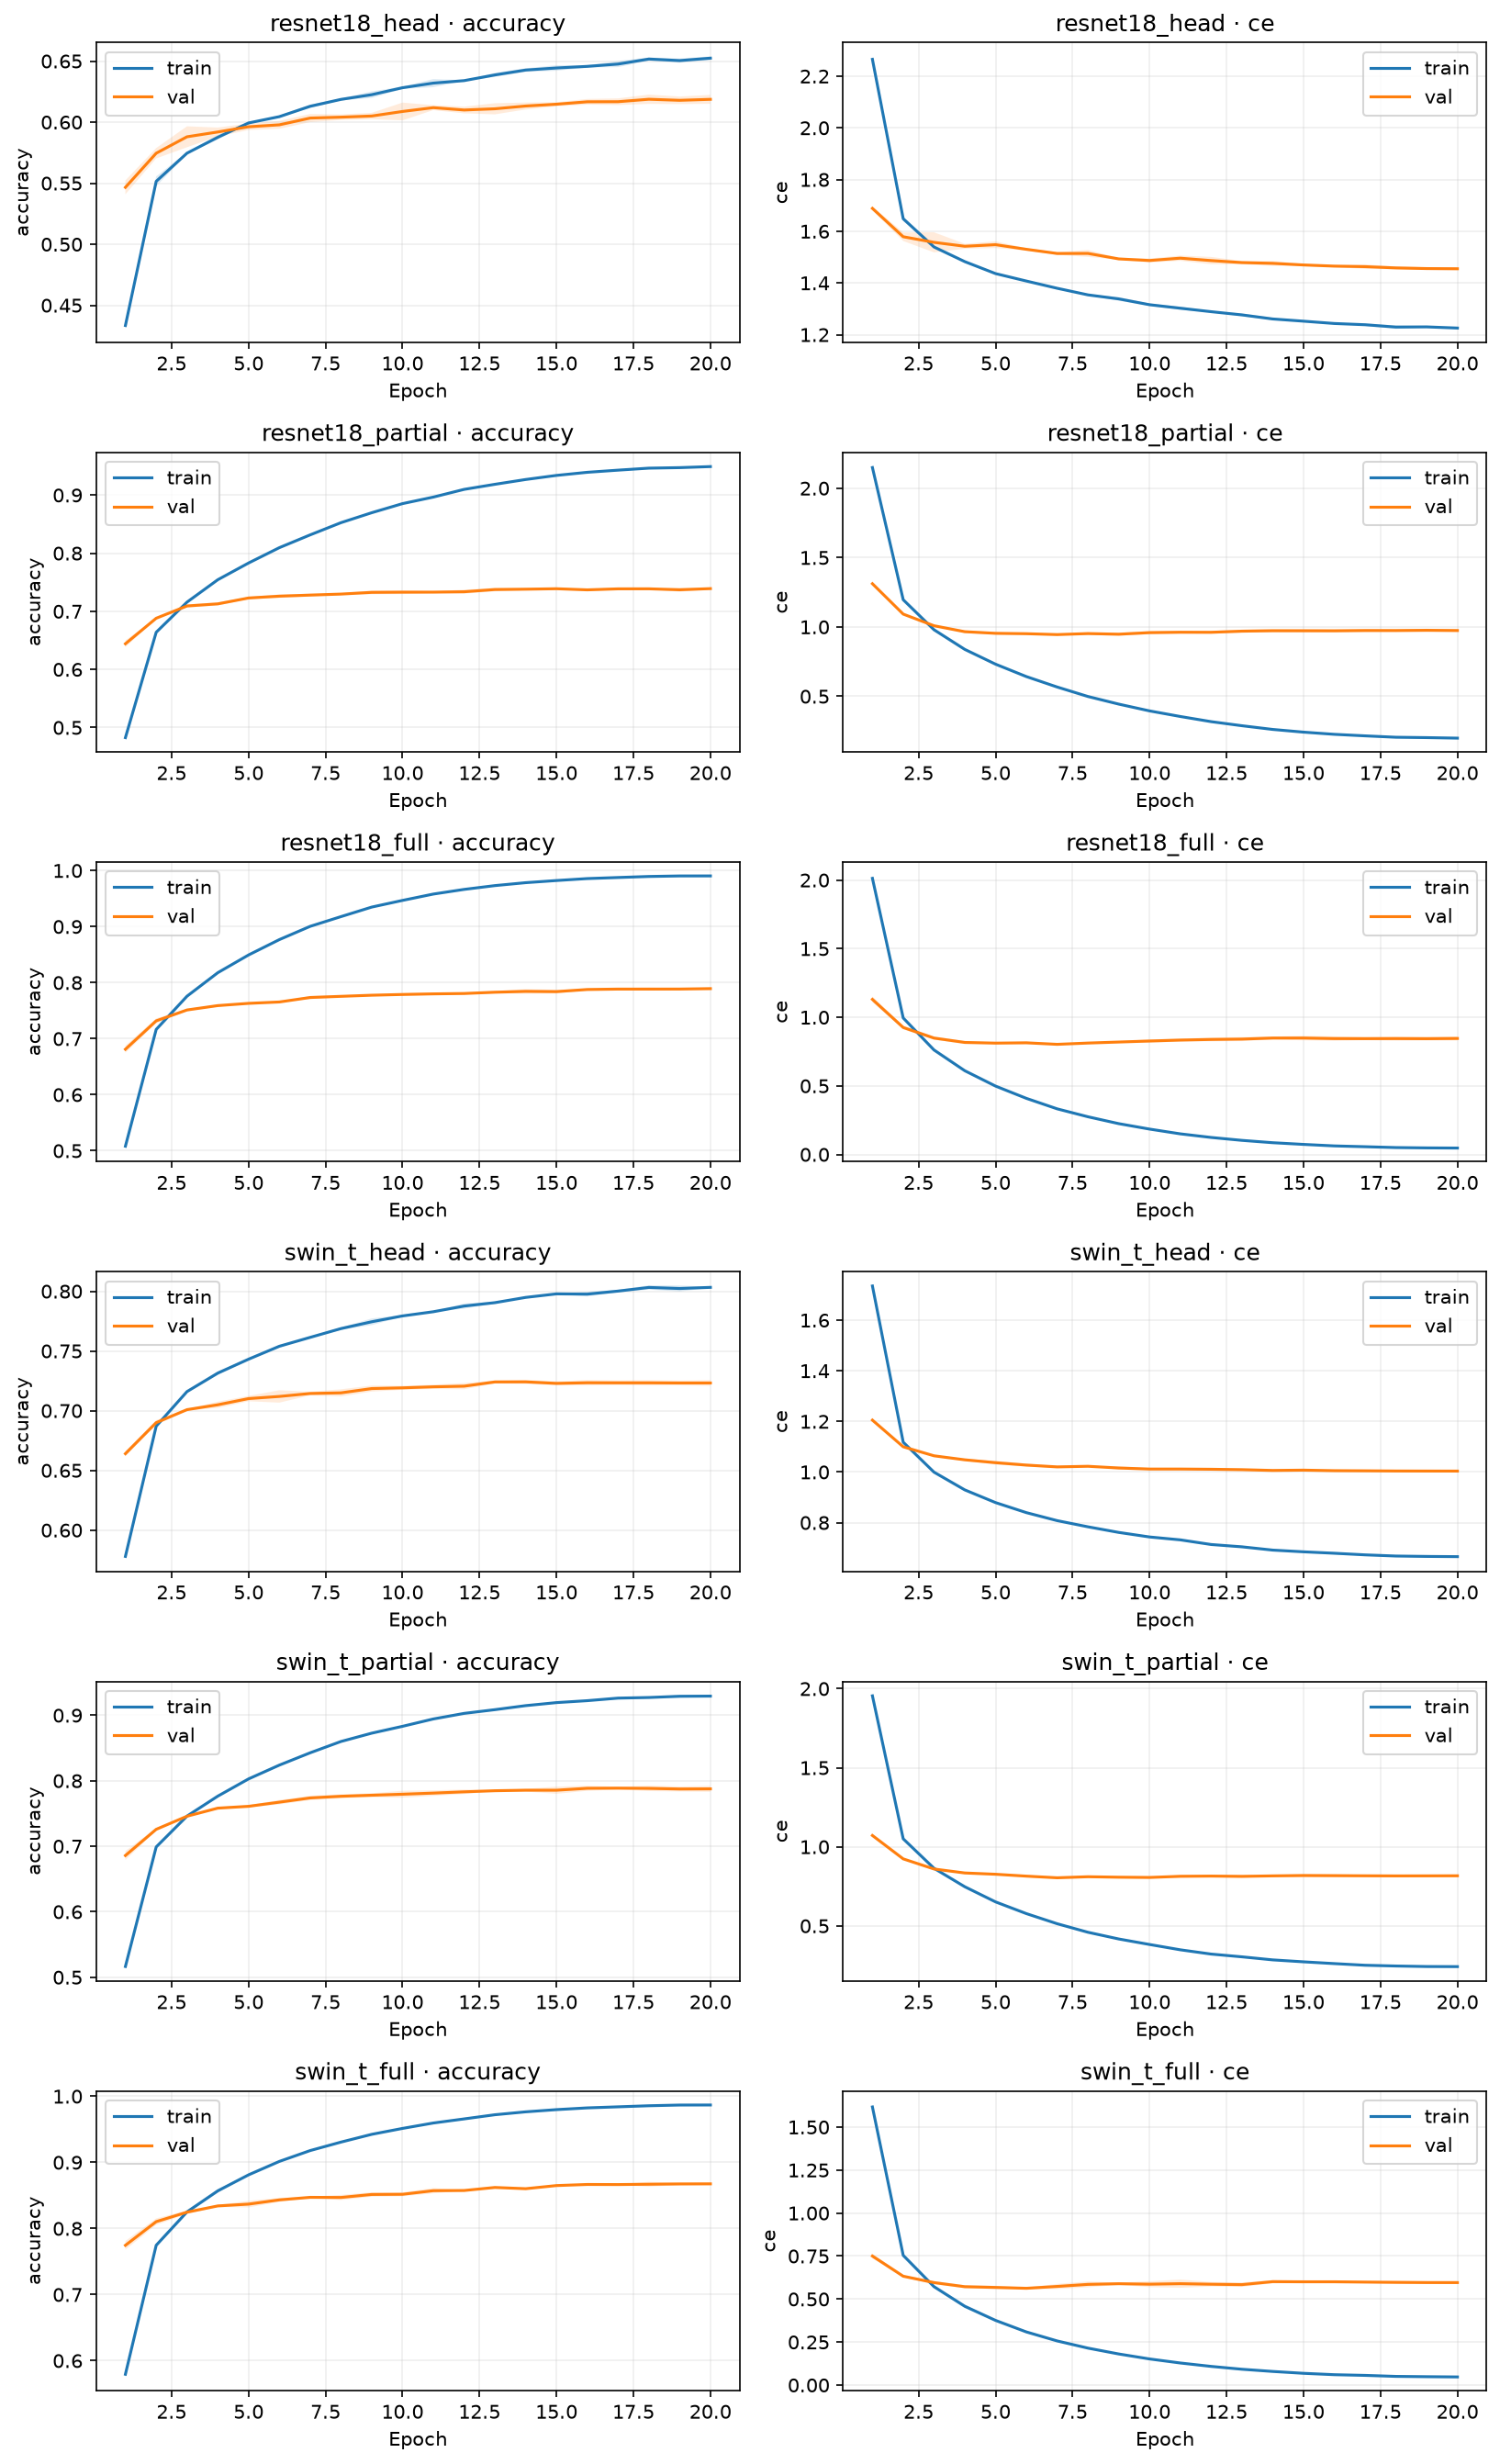
\includegraphics[trim=0 644pt 0 0,clip,width=\textwidth]{notebook-evidence/figures/learning_curves.png}
\caption{Accuracy và cross-entropy trên train/validation của ba cấu hình ResNet18 qua 20 epoch; đường cong tổng hợp từ các seed 42, 43 và 44.}
\end{figure}

\begin{figure}[htbp]\centering
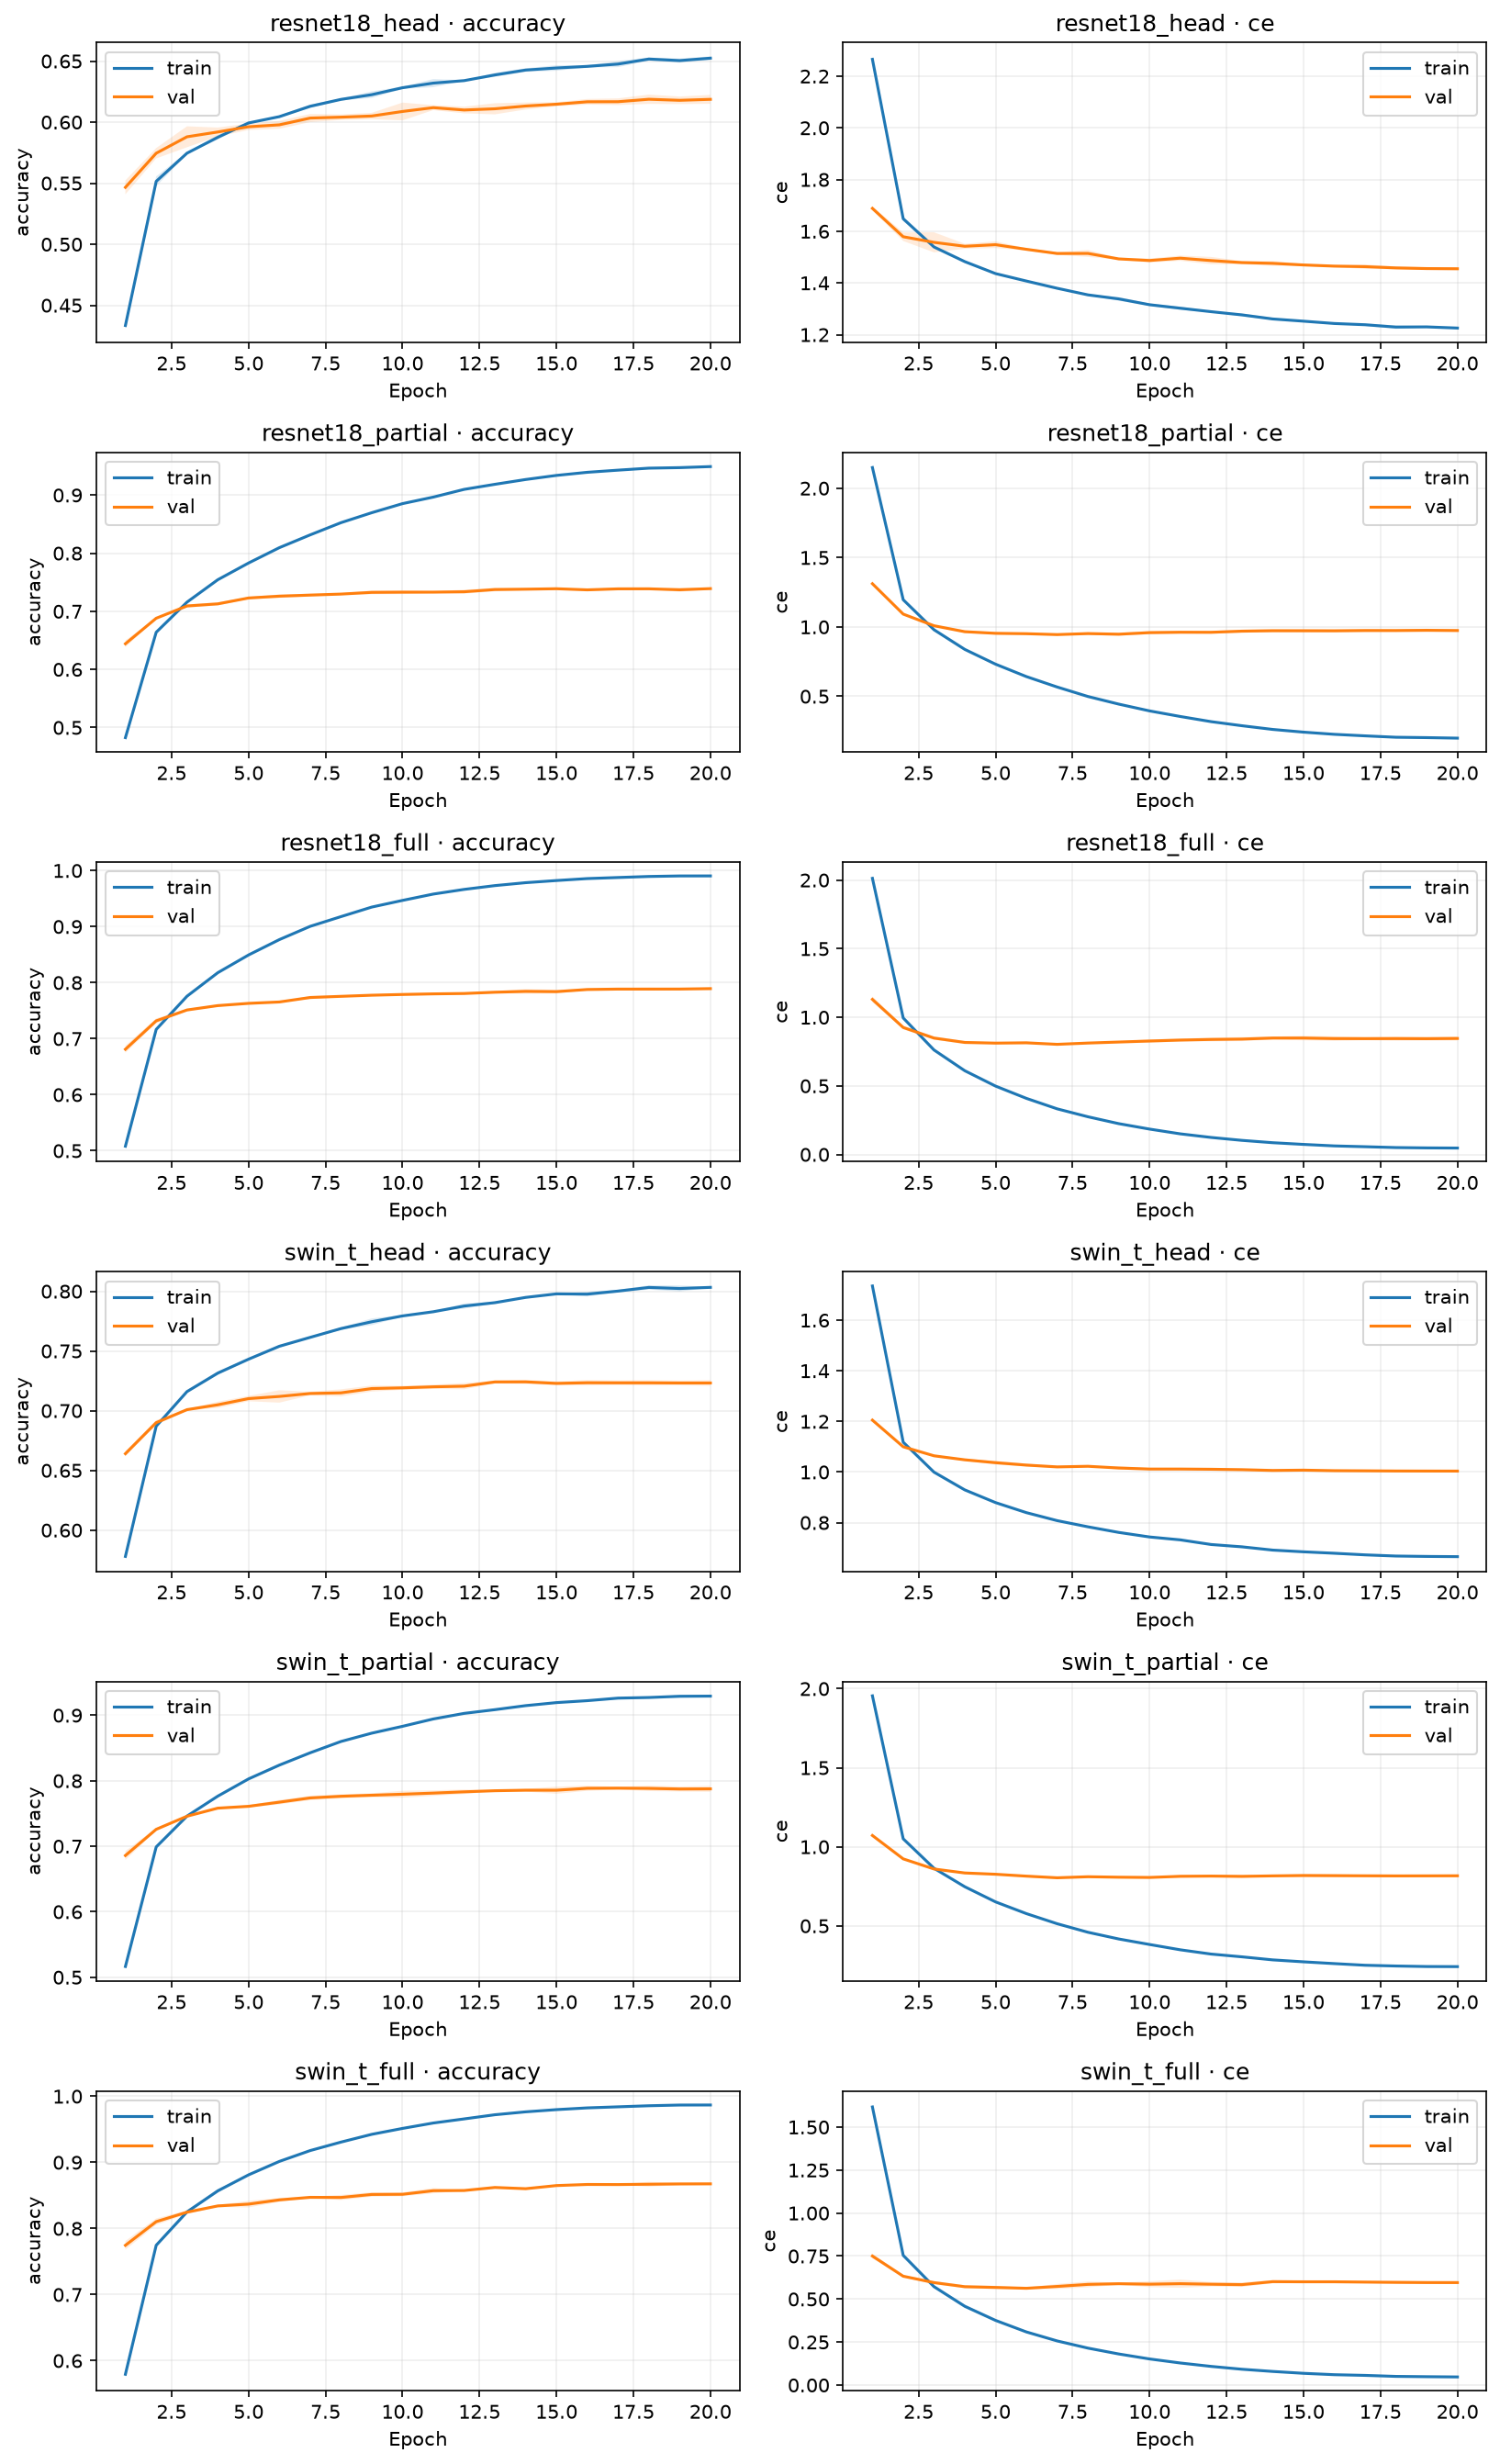
\includegraphics[trim=0 0 0 644pt,clip,width=\textwidth]{notebook-evidence/figures/learning_curves.png}
\caption{Accuracy và cross-entropy trên train/validation của ba cấu hình Swin-T qua 20 epoch; đường cong tổng hợp từ các seed 42, 43 và 44.}
\end{figure}

Các đường cong cho thấy accuracy trên tập train tiếp tục tăng trong khi mức cải thiện trên validation chậm lại. Ở epoch cuối, ResNet18 full đạt khoảng 99\% accuracy trên tập train nhưng chỉ khoảng 79\% trên validation; Swin-T full tương ứng khoảng 99\% và 87\%. Khoảng cách này cho thấy việc khớp tốt hơn với tập train không chuyển hoàn toàn thành chất lượng trên ảnh chưa dùng để cập nhật tham số. Do augmentation chỉ áp dụng trong train và số đo train được tích lũy khi tham số đang thay đổi, đây không phải phép so sánh hai tập trong điều kiện suy luận giống hệt nhau. Checkpoint vì vậy được chọn theo validation thay vì mặc định lấy epoch cuối.

\section{Chi phí và so sánh ghép cặp}

Swin-T full cao hơn ResNet18 full $7{,}66\pm0{,}41$ điểm phần trăm theo chênh lệch ghép cặp cùng seed; độ lệch chuẩn được tính từ ba chênh lệch theo seed. Macro-F1 của hai cấu hình lần lượt là $0{,}8681\pm0{,}0001$ và $0{,}7915\pm0{,}0038$.

\begin{table}[htbp]\centering\small
\begin{tabular}{lrr}
\toprule
Cấu hình & Thời gian train (s) & Peak allocated memory (MiB)\\\midrule
ResNet18 head-only & $79,0\pm0,2$ & $251,6\pm0,4$\\
ResNet18 partial & $79,5\pm0,1$ & $347,4\pm0,0$\\
ResNet18 full & $79,6\pm0,2$ & $520,4\pm0,0$\\
Swin-T head-only & $83,7\pm0,4$ & $501,9\pm0,0$\\
Swin-T partial & $104,8\pm0,1$ & $662,9\pm0,0$\\
Swin-T full & $209,6\pm0,1$ & $2454,2\pm0,0$\\
\bottomrule
\end{tabular}
\caption{Trên cùng RTX 5090 và bốn workers, Swin-T full đạt accuracy 86,81\% so với 79,16\% của ResNet18 full: mức tăng 7,66 điểm phần trăm theo ba cặp seed đi kèm 2,63 lần thời gian train và 4,72 lần bộ nhớ cấp phát cực đại. Chi phí là trung bình $\pm$ SD mẫu qua seed 42, 43 và 44; SD bộ nhớ làm tròn về 0,0 MiB ở năm cấu hình, riêng ResNet18 head-only là 0,4 MiB.}
\label{tab:new-image-cost}
\end{table}

Trong chế độ full, Swin-T mất thời gian gấp 2,63 lần và dùng peak memory gấp 4,72 lần ResNet18. Chỉ học head giảm bộ nhớ cấp phát cực đại ở cả hai backbone. Với Swin-T, thời gian train giảm từ 209,6 xuống 83,7 giây; với ResNet18, chênh lệch thời gian giữa ba mức fine-tuning chỉ khoảng 0,6 giây. Do thời gian đo bao gồm nạp dữ liệu và augmentation, không thể suy trực tiếp mức giảm phép tính backward từ mức giảm tổng thời gian này. Swin-T partial có accuracy gần ResNet18 full nhưng dùng nhiều thời gian và bộ nhớ hơn trong phép đo này; lợi thế accuracy rõ hơn của Swin-T xuất hiện ở full. Các tỷ lệ chi phí chỉ áp dụng cho cùng RTX 5090 và giao thức 20 epoch, chưa cho biết tốc độ suy luận hoặc hiệu quả trên phần cứng khác.

\section{Phân tích nhầm lẫn}

\begin{figure}[htbp]\centering
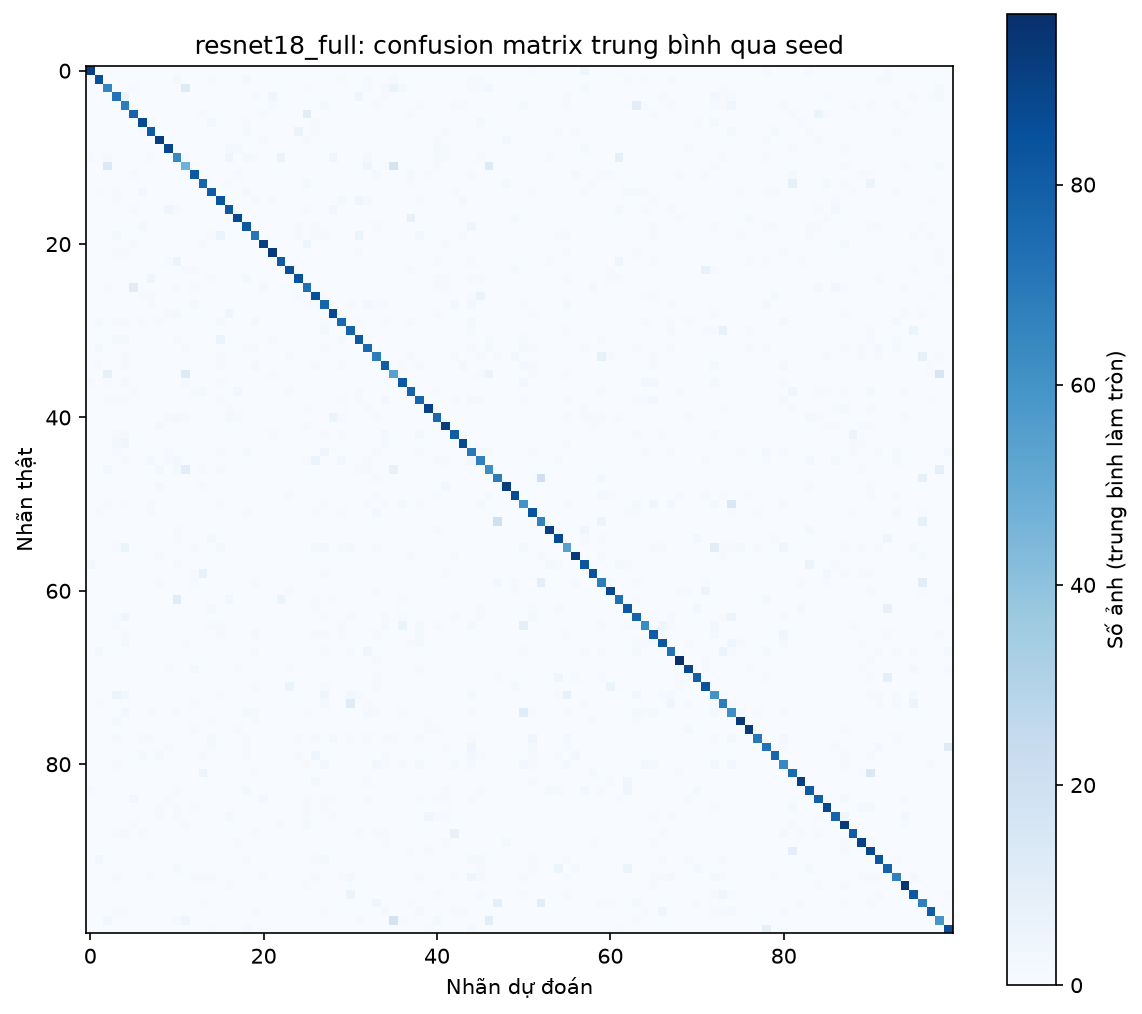
\includegraphics[width=.48\textwidth]{notebook-evidence/figures/resnet18_full-confusion.png}\hfill
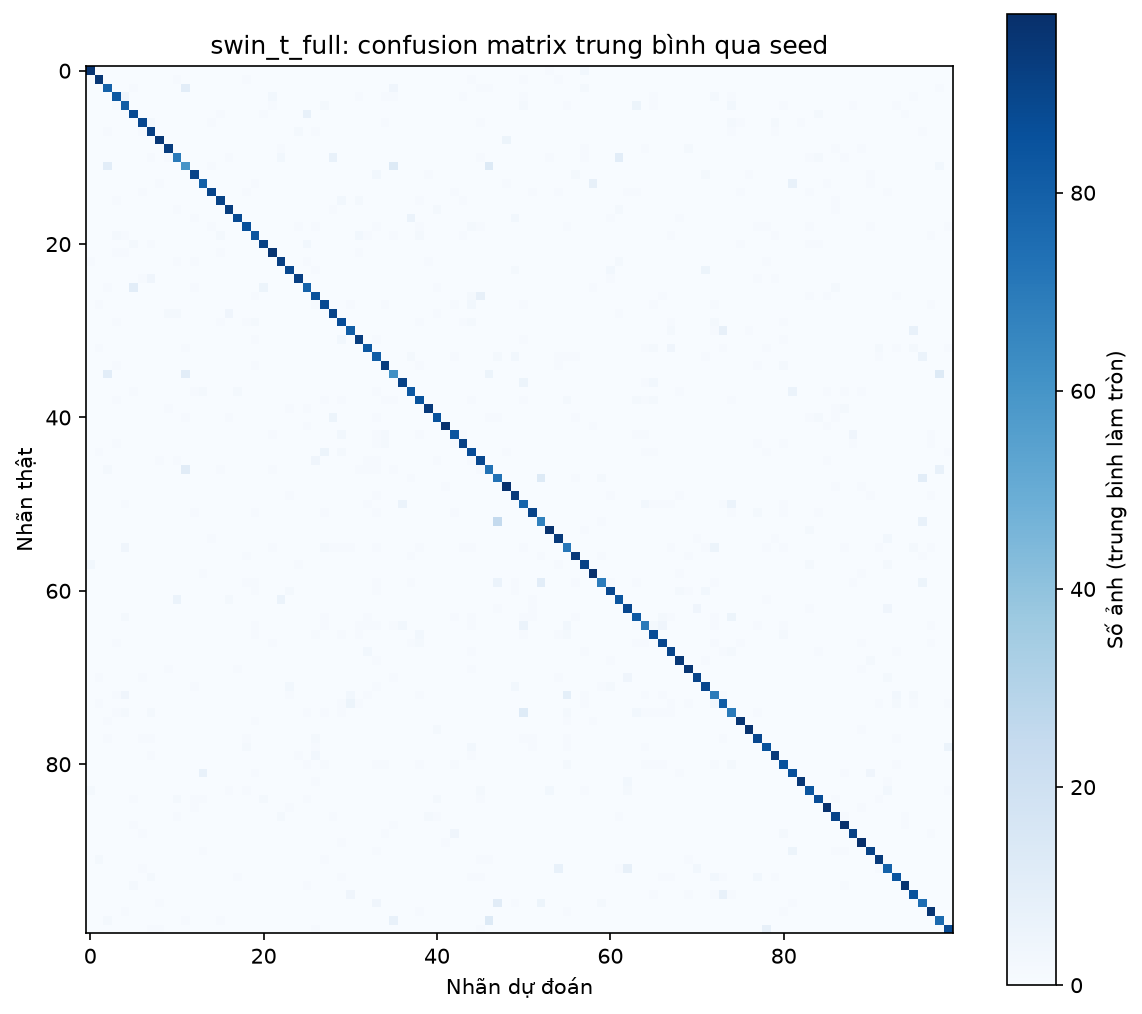
\includegraphics[width=.48\textwidth]{notebook-evidence/figures/swin_t_full-confusion.png}
\caption{Confusion matrix test trung bình qua các seed 42, 43 và 44: ResNet18 full (trái), Swin-T full (phải). Màu biểu diễn số ảnh trung bình tại mỗi ô; trục dùng chỉ số lớp từ 0 đến 99, không ghi số ảnh trong từng ô.}
\end{figure}

Trong confusion matrix, hàng biểu diễn nhãn đúng và cột biểu diễn nhãn dự đoán. Đường chéo ghi nhận dự đoán đúng, còn các ô ngoài đường chéo cho biết hướng nhầm lẫn cụ thể. Do hình gồm 100 lớp và không có nhãn tên lớp, Bảng~\ref{tab:image-confusion-pairs} bổ sung bốn hướng nhầm lẫn cùng chỉ số hàng, cột tương ứng.

\begin{table}[htbp]\centering\small
\begin{tabularx}{\textwidth}{@{}XXrr@{}}
\toprule
Nhãn đúng (hàng) & Nhãn dự đoán (cột) & ResNet18 full & Swin-T full\\\midrule
oak\_tree (52) & maple\_tree (47) & 19,00 & 23,67\\
maple\_tree (47) & oak\_tree (52) & 18,33 & 16,00\\
woman (98) & girl (35) & 16,67 & 9,67\\
girl (35) & woman (98) & 15,33 & 11,33\\
\bottomrule
\end{tabularx}
\caption{Số ảnh bị phân loại sai trung bình qua seed 42, 43 và 44 tại bốn ô ngoài đường chéo, làm tròn đến hai chữ số thập phân. Mỗi hàng là một hướng nhầm lẫn, không phải tổng hai chiều; chỉ số lớp bắt đầu từ 0 như trên hình.}
\label{tab:image-confusion-pairs}
\end{table}

Nhầm lẫn oak\_tree với maple\_tree vẫn nổi bật ở cả hai mô hình. Dù accuracy tổng thể cao hơn, Swin-T full có nhiều lỗi theo hướng oak\_tree sang maple\_tree hơn ResNet18 full, trong khi số lỗi ở chiều ngược lại thấp hơn. Với hai hướng woman--girl, số lỗi đều giảm ở Swin-T full. Như vậy, cải thiện accuracy tổng thể không đồng nghĩa với cải thiện ở mọi cặp lớp. Để giải thích các khác biệt này cần xem ảnh bị phân loại sai và so sánh đặc trưng; riêng confusion matrix chưa xác định được vai trò của độ phân giải, hình dạng vật thể hay kiến trúc.
